\chapter{Anleitung zur Nutzung des Servers und des Clients}
\label{chapter:Anleitung}

Dieses Kapitel widmet sich mit dem Umgang des Servers und der dazugeh�rigen Clients. Angef�gte Screenshots sollen einen Einblick geben, wie die Software funktioniert, auch wenn kein Computer zum Austesten der Applikation vorhanden ist.
%============== N E W  ==== S E C T I O N  ======== 
\section{Starten des Server}
\label{sec:Starting-Server}

Der Server ist das Herzst�ck der Applikation. Er ist so ausgelegt, dass er mit g�ltigen Argumenten erweitert werden kann.\\
Momentan gibt es zwei implementierte Argumente, welche beim Start mitgegeben werden k�nnen:
\begin{itemize}
\item \flqq -l\frqq\ -- Loglevel\\
F�r das Loglevel g�ltige Eingaben sind Integer mit Werten von 0-7.\\
Wird ein ung�ltiger Wert gr�sser als 7 eingegeben, wird der Fehler abgefangen und das Loglevel wird auf den default-Wert = 5 gesetzt.

\item \flqq -p\frqq\ -- Serverport\\
F�r den Server-Port g�ltige Eingaben sind: 1024 - 65535. Die well-known Ports von 1 - 1023 wurden bewusst nicht erlaubt, da es Konflikte geben k�nnte mit anderen Applikationen.\\
Wird ein ung�ltiger Wert eingegeben, wird der Server automatisch mit dem default-Port = 7000 starten.
\end{itemize}

Beispiele f�r g�ltiges Starten des Servers:\\
./Server -p 4637 -l 7\\
./Server -l 6 -p 5479\\
./Server -p 7788\\
./Server -l 8\\

Die Abbildung \ref{fig:Starting_Server} zeigt einen g�ltigen Serverstart. Bei der Abbildung \ref{fig:Starting_Server2} ist zu sehen, wie das Loglevel 8 nicht gesetzt werden kann und wie die nachtr�glichen Argumente (Duplikate) des Serverports und des Loglevels ignoriert werden.

\newpage
\begin{figure}[h!]
\centering
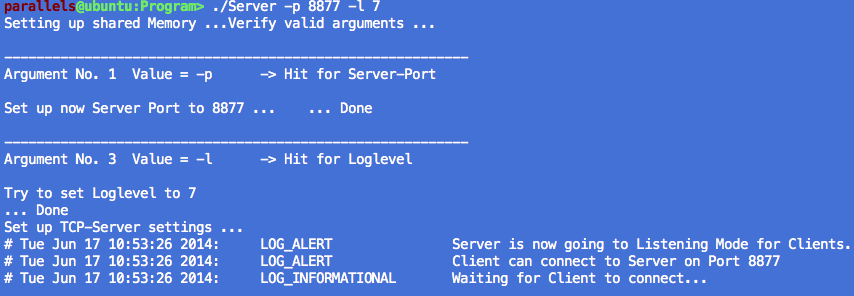
\includegraphics[width=1\textwidth]{Starting_Server.png} 
\caption[Starten des Servers]{Starten des Servers\\Quelle: eigener Screenshot}
\label{fig:Starting_Server}
\end{figure}

\begin{figure}[h!]
\centering
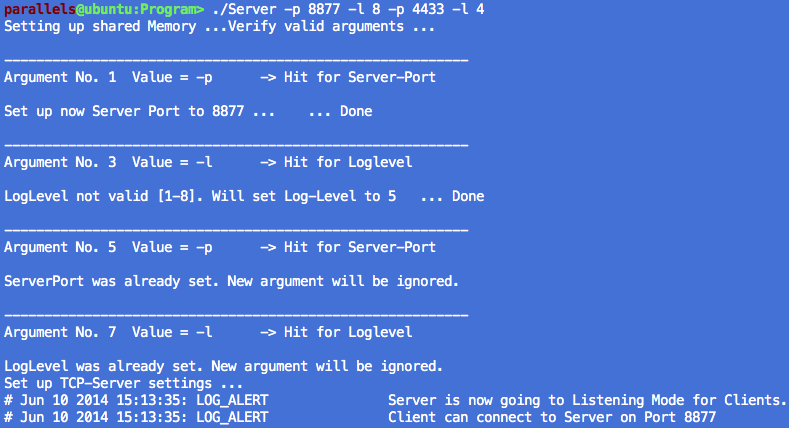
\includegraphics[width=1\textwidth]{Starting_Server2.png} 
\caption[Starten des Servers mit doppelten Argumenten]{Starten des Servers mit doppelten Argumenten\\Quelle: eigener Screenshot}
\label{fig:Starting_Server2}
\end{figure}

\textbf{Anmerkung:}\\
Die Reihenfolge der Argumente ist egal. Wird ein Argument zwei mal eingegeben (z.B. ./Server -p 7524 -l 6 -l 8), wird nur das erste Argument ber�cktsichtigt. Alle weiteren Argumente werden ignoriert.\\
./Server -p 5432 -l 5 -l 8 wird somit den TCP Port 5432 und das Loglevel 5 setzen.\\
./Server -p 2066 -p 5432 -l 4 -l 8 wird somit den TCP Port 2066 und das Loglevel 4 setzen.
%============== N E W  ==== S E C T I O N  ======== 
\newpage
\section{Starten der Clients}
\label{sec:Starting-Clients}

Der Client besitzt im Gegensatz zum Server eine sehr eingesch�nkte Logik. Seine Aufgabe besteht haupts�chlich darin, sich �ber einen TCP-Socket mit dem Server zu verbinden. \\
Beim Client ist es notwendig, die Argumente in der richtigen Reihenfolge einzugeben. So ist nur folgender Aufruf g�ltig:\\
./Client <IP Adresse von Server>\\
oder\\
./Client <IP Adresse von Server> <TCP Port Server>\\
Wird die Variante ohne den Port gew�hlt, versucht sich der Client �ber den default Port = 7000 mit dem Server zu verbinden.

\begin{figure}[h!]
\centering
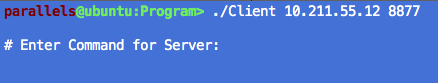
\includegraphics[width=0.5\textwidth]{Starting_Client.png} 
\caption[Starten des Clients]{Starten des Clients\\Quelle: eigener Screenshot}
\label{fig:Starting_Client}
\end{figure}

Beispiele f�r g�ltiges Starten des Clients:\\
./Client 10.211.55.12\\
./Client 10.211.55.12 5542


%============== N E W  ==== S E C T I O N  ======== 

\section{Benutzen der Clients}
\label{sec:Using-Clients}

Um die Funktionalit�ten des Servers nutzen zu k�nnen, m�ssen die Befehle vom Client zum Server gesendet werden. Direkte Eingaben im Server sind nicht zul�ssig.\\
Die g�ltigen Server-Befehle werden hier nicht erl�utert, sondern nur wie die Befehle genutzt werden k�nnen. Einen Einblick in die Implementierung der CRUD-Befehle gibt das Kapitel \ref{sec:Server-Befehle}.

\begin{itemize}
\item CREATE
\item READ
\item UPDATE
\item DELETE
\item LIST shm 
Der LIST zeigt das momentan vorhandene Shared-Memory an, wobei zu beachten gilt, dass hier kein Locking-Verfahren eingesetzt wurde. Das heisst, das Memory k�nnte bereits bei der Ausgabe auf der Konsole beim Client bereits wieder ver�ndert worden sein.
\end{itemize}






